The architecture consists of three containers being a controller, keyboard teleoperation, and a simulator. The simulator runs a Gazebo world that supports multiple 3DR Iris Quadrotor \acsp{uav} with each a PX4 Autopilot. The controller sends MAVROS commands to the \acsp{uav} for arming and changing their mode to \textit{OFFBOARD}. The \textit{OFFBOARD} mode provides full control of the \acsp{uav} through Python code. In the keyboard teleoperation container, pressed keys are parsed to the controller where they are translated to commands and send to the \acsp{uav}.

\begin{figure}[!h]
  \centering
  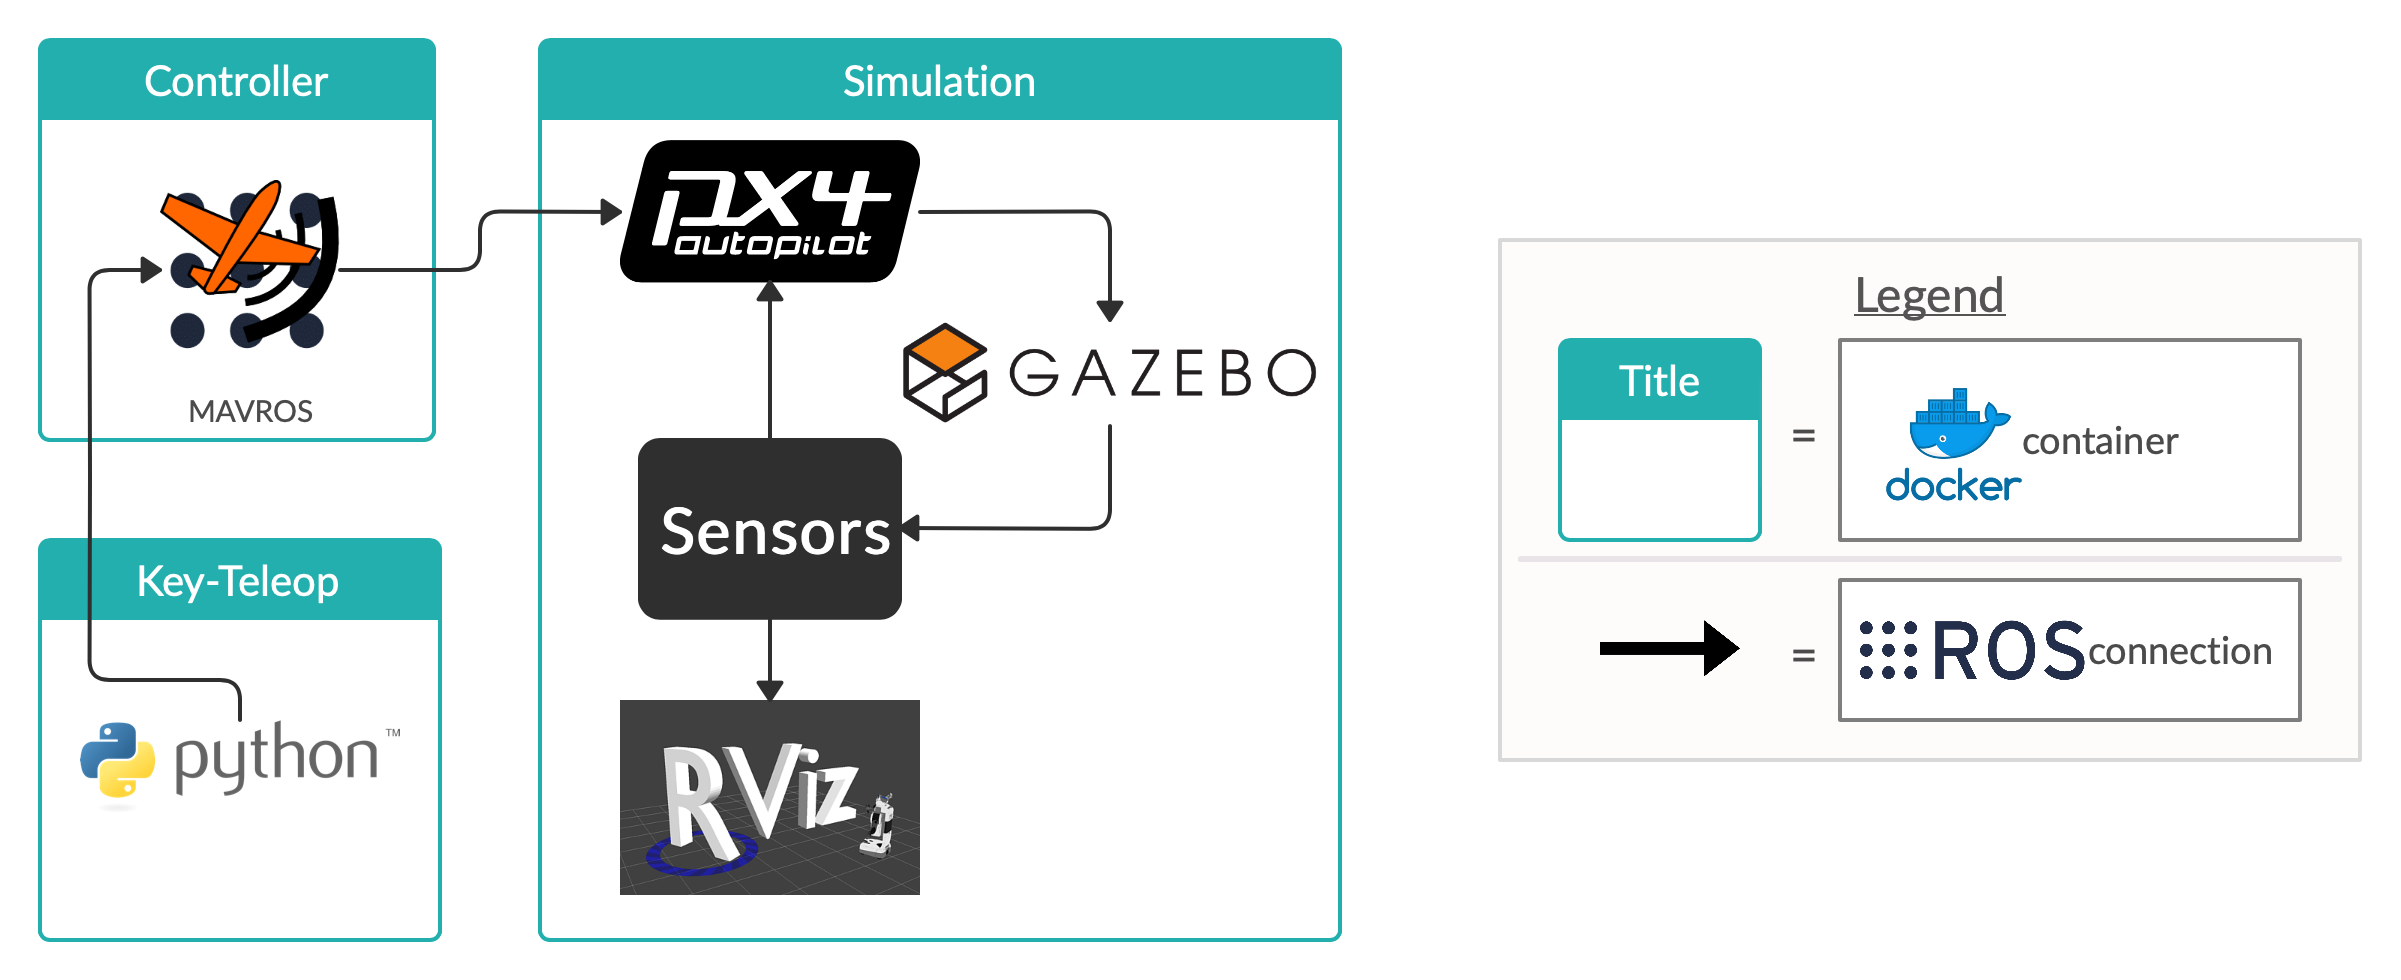
\includegraphics[width=
  \linewidth]{images/architecture_containers.png}
  \caption{Docker containers architecture}
\end{figure}

\clearpage

The containers in the architecture are run from different images. The simulation image has an \acs{opengl} base image or a specific NVIDIA base image if the host computer has NVIDIA installed. Adding to this base image, the simulation has \acs{ros} Melodic, MAVROS, Gazebo 9, the PX4 Firmware and their dependencies installed. There are two other images used in this project, a \acs{ros} base image and a MAVROS image. The keyboard teleoperation container uses the \acs{ros} base image with only \acs{ros} Melodic installed. The controller needs MAVROS to send commands to the \acsp{uav} and therefore uses the MAVROS image that extends from the \acs{ros} base image with the installation of MAVROS.

\begin{figure}[!h]
  \centering
  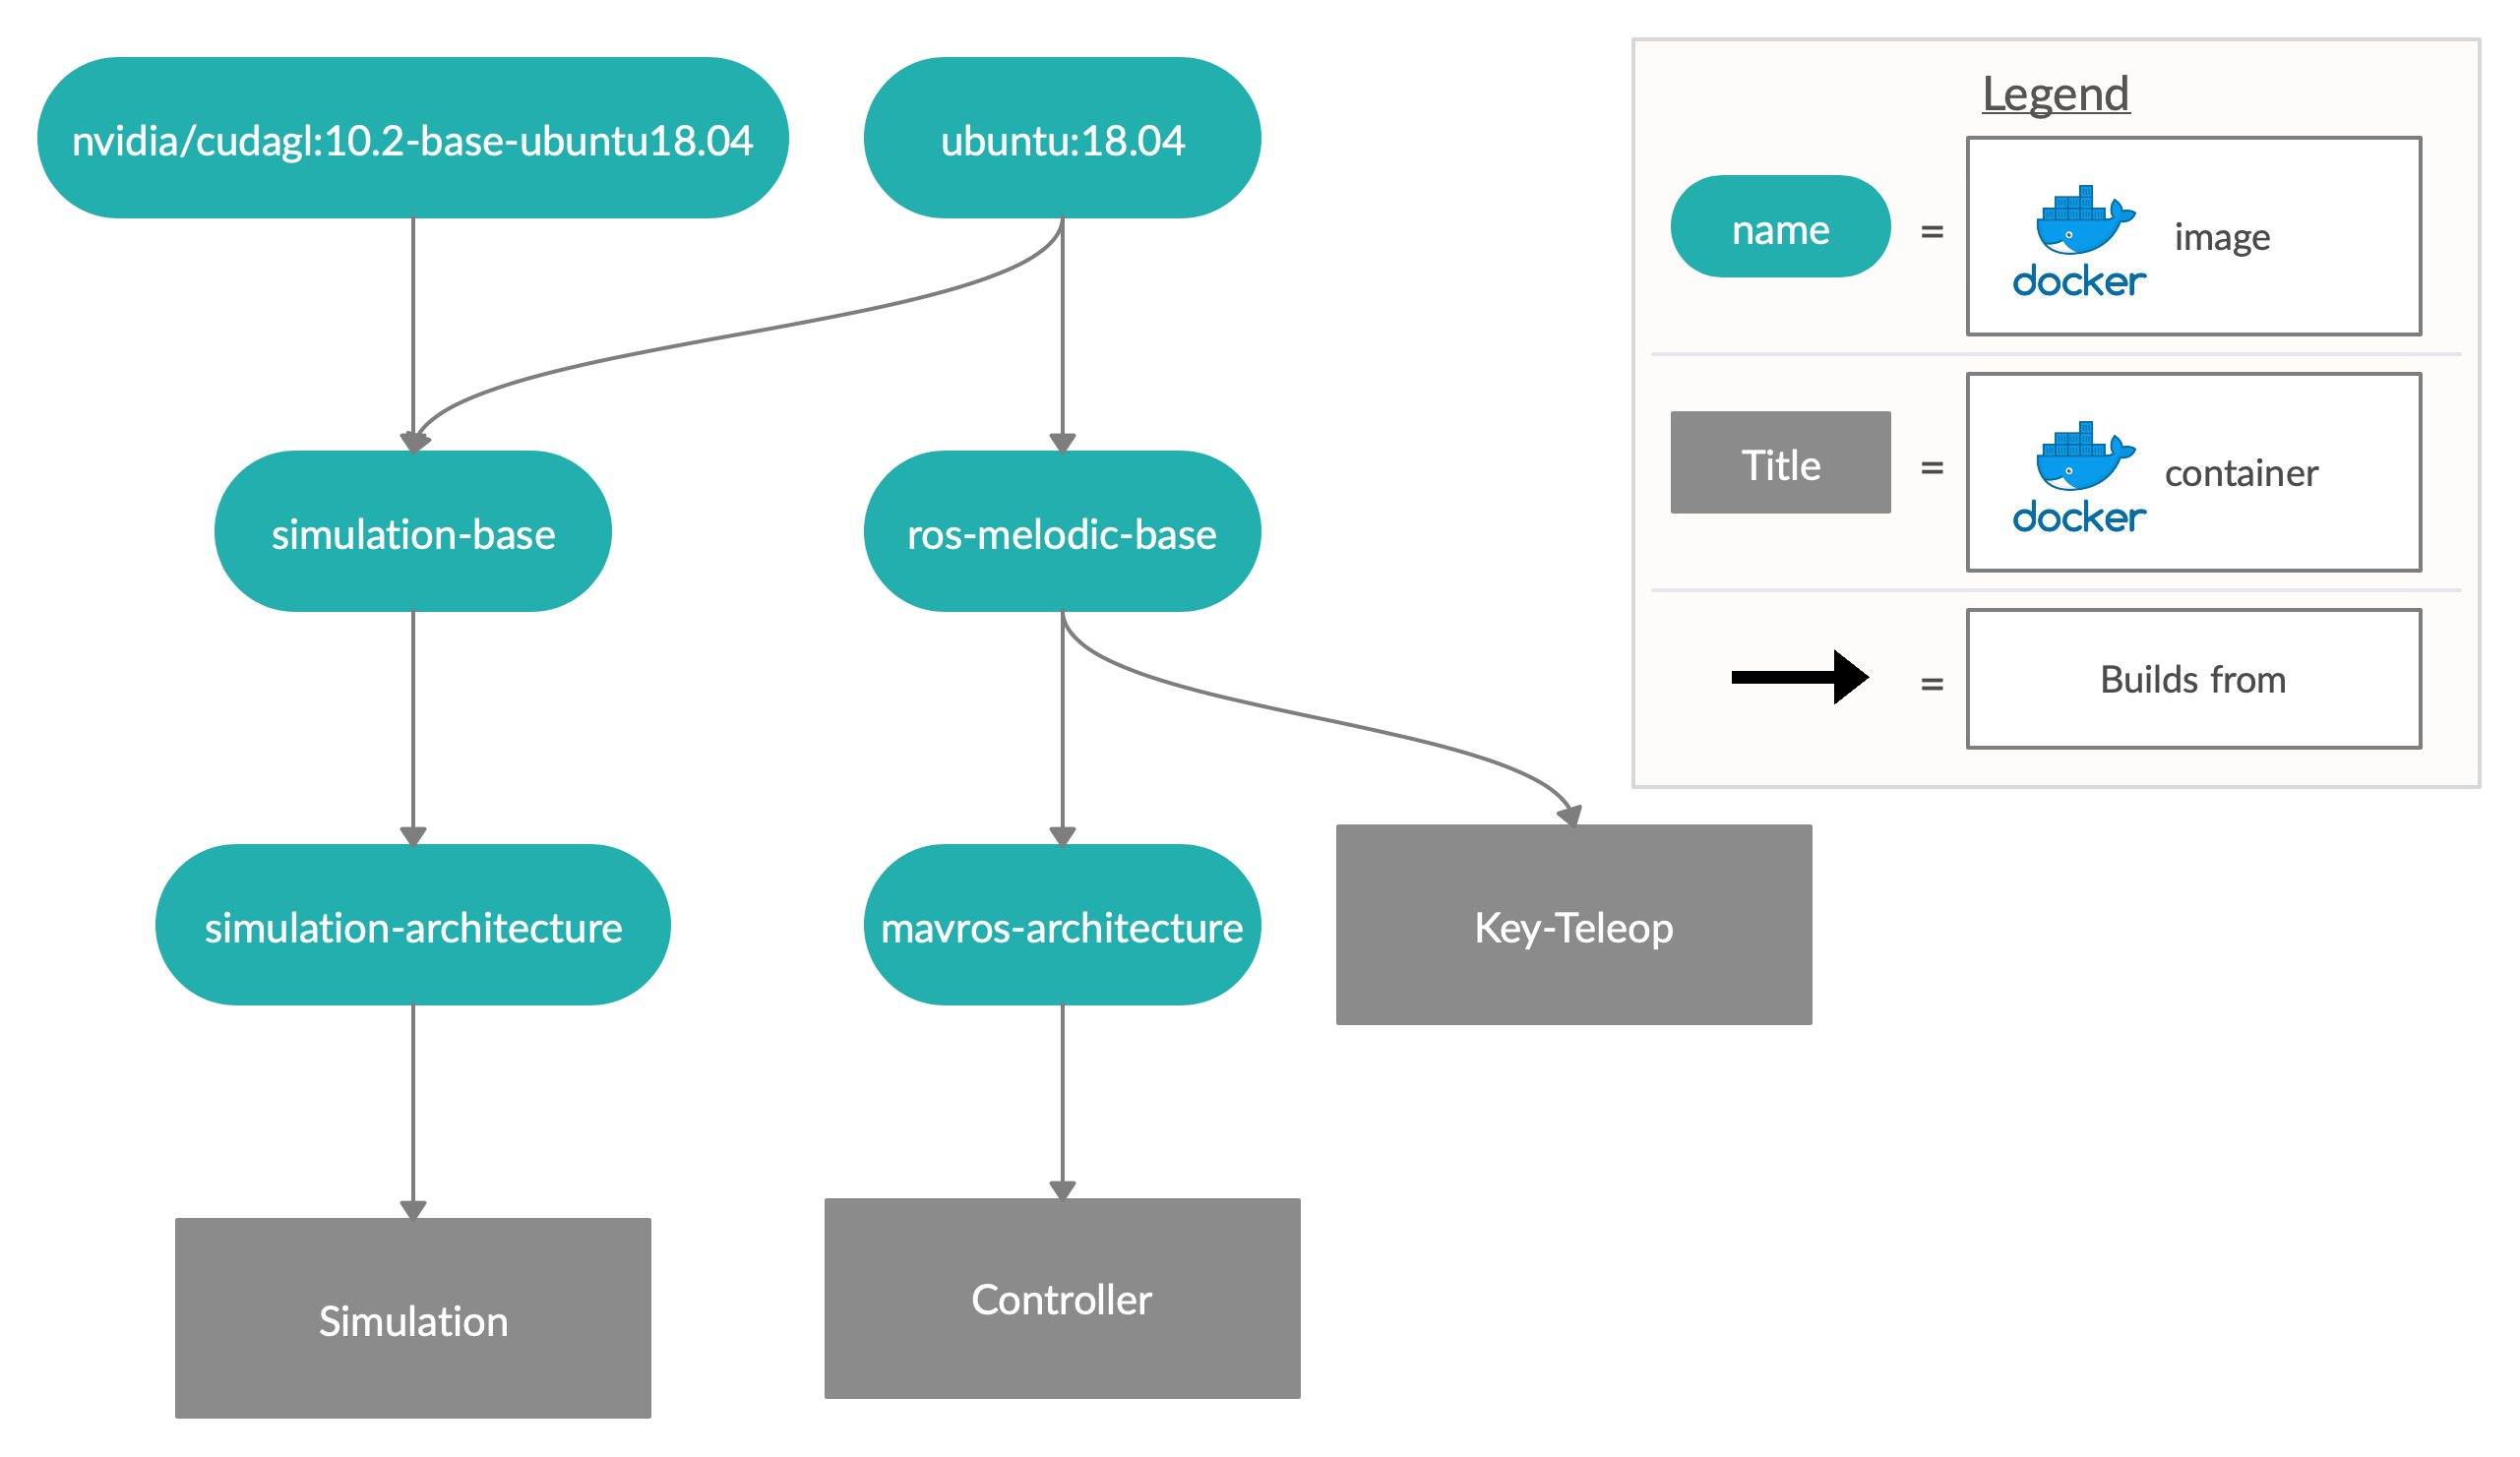
\includegraphics[width=\linewidth]{images/architecture_images.png}
  \caption{Docker images architecture}
\end{figure}

The goal of the architecture is to enable developers to develop \acs{uav} applications without having to create a workspace or installing software manually. The repository contains scripts to automate all commands to build, run and stop the containers necessary for the development. The architecture supports \acs{uav} and multi\hyp{}\acs{uav} applications.